\documentclass[10pt]{article}

% Transactions on Machine Learning Research (TMLR) Style
% Use \usepackage{tmlr} for anonymous submission to OpenReview
% Use \usepackage[preprint]{tmlr} for arXiv preprints
% Use \usepackage[accepted]{tmlr} for camera-ready publication
\usepackage{tmlr}

% Core mathematics, symbols, and formatting
\usepackage{amsmath,amssymb,amsfonts,amsthm,bm}
\usepackage{graphicx}
\usepackage{booktabs}
\usepackage{tabularx}
\usepackage{multirow}
\usepackage{array}
\usepackage{url}
\usepackage{hyperref}
\hypersetup{hidelinks}
\usepackage{color}
\usepackage{subcaption}
\usepackage{microtype}
\setlength{\textfloatsep}{7pt plus 1pt minus 1pt}
\setlength{\floatsep}{6pt plus 1pt minus 1pt}
\setlength{\intextsep}{6pt plus 1pt minus 1pt}
\setlength{\abovecaptionskip}{3pt plus 1pt minus 1pt}
\setlength{\belowcaptionskip}{0pt}

% Mathematical notation macros
\newcommand{\E}{\mathbb{E}}
\newcommand{\R}{\mathbb{R}}
\newcommand{\loss}{\mathcal{L}}
\newcommand{\dataset}{\mathcal{D}}
\newcommand{\EffRank}{\mathrm{EffRank}}
\newcommand{\Dcka}{D_{\mathrm{CKA}}}
\newcommand{\vtheta}{\bm{\theta}}
\newcommand{\urec}{u_{\mathrm{rec}}}

\title{Transient Collapse and Asymptotic Plasticity: How Procedural Resets Confound Auxiliary Transfer in Deep Vision}

\author{\name Vishesh Panghal \email pvt.panghal@gmail.com \\
      \addr Department of Artificial Intelligence and Data Science\\
      Poornima Institute of Engineering and Technology, Jaipur, India
      \AND
      \name Lakhan Bhaskar Kadel \email Lbhaskar@iujaipur.edu.in \\
      \addr Department of Computer Science and Engineering\\
      The ICFAI University, Jaipur, India
      \AND
      \name Shalini Pathak \email shalini.pathak@jaipur.manipal.edu \\
      \addr School of Computer Science and Engineering\\
      Manipal University Jaipur, India}

\def\month{11}
\def\year{2026}
\def\openreview{Draft}

\begin{document}

\maketitle

\begin{abstract}
Switching a vision model to an intermediate dataset often changes its target accuracy. Because the switch also replaces the classification head and resets optimizer momentum, the accuracy change is difficult to attribute to the auxiliary data alone. We examine the auxiliary-data and procedural contributions under matched computational budgets in two settings. A ResNet-18 trained from scratch on CIFAR-100 takes an STL-10 detour ($N = 20$ paired seeds). An ImageNet-pretrained ResNet-50 fine-tuned on clinical dermoscopy images (ISIC 2019) takes a natural image detour ($N = 8$ paired seeds). In the from-scratch setting, taking an auxiliary detour yields an average test accuracy of 56.26\%, while uninterrupted training reaches 56.69\% (a gap of $-0.43$ percentage points, $p = 0.090$). A procedural reset control ($C_3$), which performs the same head swap and momentum reset on target data alone, shows the same shortfall (56.29\%, $-0.40$ percentage points vs.\ $C_0$, $p = 0.269$). A $2 \times 2$ factorial experiment confirms that replacing the prediction head causes this performance drop ($-2.10$ percentage points, $p = 0.004$), while clearing momentum buffers provides a small regularizing benefit ($+0.57$ percentage points, $p = 0.279$). In the clinical transfer setting, off-task updates temporarily reduce feature dimensionality, causing Effective Rank to drop from 1147 to 787 dimensions ($p < 10^{-11}$). However, resuming target training fully restores feature geometry, leading to statistical parity across all conditions ($C_0$: 85.18\%, $C_3$: 84.68\%, $S_1$: 84.76\%; $p = 0.767$). The accuracy comparisons demonstrate that performance drops during multi-phase training reflect the disruption of optimizer and head resets rather than negative data transfer. Deep neural representations show strong plasticity, recovering their structure once target training resumes.
\end{abstract}



\section{Introduction}\label{sec:intro}

Training a deep vision model often involves several tasks before final evaluation. Intermediate supervised tasks, self-supervised objectives, and auxiliary datasets are commonly used to improve what the model learns from its training data \cite{caruana1997multitask,phang2018stilts,pruksachatkun2020intermediate,kirkpatrick2017overcoming,rebuffi2017icarl,davari2022probing}. The expectation is that features acquired on another task may help the target problem, especially when labeled target data are limited \cite{yosinski2014transferable,aghajanyan2021muppet}. Yet an accuracy change after auxiliary training does not identify how much the additional examples contributed.

For a CIFAR-100 model that temporarily trains on STL-10 before returning to CIFAR-100, auxiliary images, head management, optimizer state, and target exposure change together. Different label spaces require a separate classification head; optimizer state may also change at the task boundaries. Under a constant update budget, each period that is allocated to STL-10 training constitutes a period of training of CIFAR-100. The control scheme involves the same head swapping and momentum initialization without the use of any other dataset, making it possible to compare the two schemes.





\subsection{The Budget Distinction: Total Updates vs. Target Updates}\label{subsec:intro_budgets}

The difference between the two budget comparisons is in what is being matched the total number of updates ($\Delta_{\mathrm{total}}$) or the target exposure ($\Delta_{\mathrm{target}}$). In terms of total budget $u_{\mathrm{total}}=35{,}000$, a 5,000 update detour $S_1$ has 30,000 target updates while continuous training $C_0$ has 35,000. However, matching the target exposure yields 30,000 target updates for both schedules and treats the detour as additional compute.

Matching target exposure alone confuses transfer learning with extra training steps. Matching total updates removes that ambiguity; the on-target procedural control ($C_3$) is still needed to distinguish auxiliary data effects from the shock of resetting the optimizer.

\subsection{Summary of Empirical Findings}\label{subsec:intro_contributions}

We establish three main findings across from-scratch pretraining and transfer fine-tuning. At fixed total compute, auxiliary detours do not improve target generalization. On CIFAR-100 ($N = 20$ paired seeds), the STL-10 detour ($S_1$) reaches 56.26\% mean test accuracy, compared with 56.69\% for continuous training ($C_0$; a $-0.43$ percentage point difference, $p = 0.090$). Resetting the head and momentum on CIFAR-100 alone produces almost exactly the same deficiency of the on-target procedural control ($C_3$), at 56.29\% accuracy (a $-0.40$ percentage point drop compared to $C_0$, $p = 0.269$). The difference between the detour and the on-target control procedure is essentially nonexistent (-0.03 percentage points, $p = 0.941$), proving that the decrease in accuracy results from the resetting procedure itself, not from any negative transfer effects.

We employed a $2 \times 2$ factorial design where $N = 6$ paired seeds were used to distinguish between the head and momentum effects that are packaged into one $C_3$. The two effects can be independently varied to distinguish their individual effects, which cannot be done if they are reset together. Head substitution gave a $-2.10$ percentage point effect ($p = 0.004$). Momentum clearing gave a positive estimate of $+0.57$ percentage points ($p = 0.279$), but the evidence was insufficient to establish an improvement. The interaction estimate was small ($+0.02$ percentage points, $p = 0.967$). Head substitution was the more substantial source of accuracy loss within this six-seed experiment.

Pretrained representations undergo acute temporary collapse during off-task updates. They recover fully during target relearning. When fine-tuning ImageNet-pretrained ResNet-50 models on clinical dermoscopy (ISIC 2019, 25,331 images across $N = 8$ paired seeds), an off-task natural image detour reduces Effective Rank from 1147 to 787 dimensions ($p < 10^{-11}$) and sharply increases CKA drift ($p < 10^{-7}$). Resuming target training completely reverses this geometric collapse. All experimental arms reach statistical parity at the end of training ($C_0$: 85.18\%, $C_3$: 84.68\%, $S_1$: 84.76\%; $p = 0.767$). Pretrained vision features thus have broad basins of attraction and can absorb severe short-term distortion without losing their ability to generalize to the target task.

\section{Related Work}\label{sec:related_work}

\subsection{Auxiliary and Intermediate-Task Learning}\label{subsec:related_auxiliary}
Intermediate-task fine-tuning (STILTs) \cite{phang2018stilts,pruksachatkun2020intermediate} and multi-task interleaving \cite{davidson2020sequential,mayo2023multitask} commonly introduce other tasks between pretraining and target fine-tuning. Their benefits depend on the auxiliary data: large datasets closely related to the target can help, whereas domain shift and small sample sizes often reduce or reverse the benefit \cite{yosinski2014transferable,aghajanyan2021muppet}. Earlier studies rarely fix total parameter updates across baseline and detour models. Reported gains therefore have two possible explanations: transfer from the intermediate task or additional optimization steps.

\subsection{Continual Learning and Optimization Restarts}
\label{subsec:related_continual}

The learning of task $B$, after learning task $A$, can negatively affect some of the parameters which were helpful for learning task $A$ because of interference and lead to forgetting of the previously learned information \cite{mccloskey1989catastrophic,french1999catastrophic,kirkpatrick2017overcoming,lopezpaz2017gem}. Most of the forgetting studies measure how much forgetting takes place after changing tasks. Our problem statement is concerned about how $A$ can be carried out after learning $B$. More specifically, do the representations which are now forgotten have any purpose or can they be relearned? The transitions between the tasks can affect the optimization conditions. The learning rate restarts and the cyclic scheduling are optimization techniques by themselves \cite{loshchilov2017sgdr,smith2017cyclical}. The head replacements and momentum clearing play this role in our case and hence make it hard to attribute any accuracy difference to just the intermediate task. The procedural control ($C_3$) keeps the training on task $A$ with the same head swaps and momentum resets as in the auxiliary schedule, thus helping to differentiate between the auxiliary-data effects and the transition effects.


\subsection{Representation Geometry and Latent Auditing}
\label{subsec:related_probing}

Accuracy of the final test may obscure both distinctions among the representations used internally by the model and significant changes that take place during the training process. Adding an auxiliary interval could distort target representations, even if later target fine-tuning recovers much of the loss in performance. We analyze representations just before the target task using linear probing classification \cite{alain2017understanding,belinkov2022probing}, Centered Kernel Alignment (CKA) \cite{kornblith2019similarity}, and Effective Rank ($\EffRank$) \cite{roy2007effective,begga2026preserving}. Linear probing measures how well a frozen backbone contains information about target-class distinctions usable by a linear classifier. In turn, CKA measures how representations change over time while Effective Rank ($\EffRank$) describes the spread of feature matrix singular values: a reduction in Effective Rank indicates that variation is concentrated along fewer dimensions. Using compute-matched baselines, these distinct measurements allow separating changes in representation brought by auxiliary training and later recovery. The recovery of target accuracy does not necessarily guarantee the restoration of the earlier representation.


\section{Schedule Definitions, Transition Rules, and Estimands}\label{sec:schedules}

\subsection{Multi-Phase Schedule Formulation}\label{subsec:schedule_formulation}

The total number of parameter update steps is established by a common three-step budget $u_{\mathrm{total}} = u_1 + u_B + u_2$. During the first step, the backbone and target head $\bm{\theta}_{\mathrm{bb}}$, $h_A$ are trained on the dataset $\mathcal{D}_A$ for $u_1$ steps. The checkpoint $\bm{\theta}_1$ saved at the end of Phase 1 will be the common starting point for all the conditions. Starting from $\bm{\theta}_1$, we split the schedule into different trajectories in Phase 2 ($u_B$ steps). Continuous baseline ($C_0$) proceeds training on $\mathcal{D}_A$ without changes. Procedural reset control ($C_3$) also trains on $\mathcal{D}_A$, but it changes the head and erases momentum from the optimizer. Auxiliary detour ($S_1$) trains on $\mathcal{D}_B$ and uses a new head $h_B$. The second checkpoint $\bm{\theta}_2$ is saved after $u_1 + u_B$ steps, and their representations and weights are checked. All the schedules train on $\mathcal{D}_A$ for $u_2$ steps in Phase 3. Before that, we restore the target head $h_A$ for $C_3$ and $S_1$.

\begin{figure*}[t]
\centering
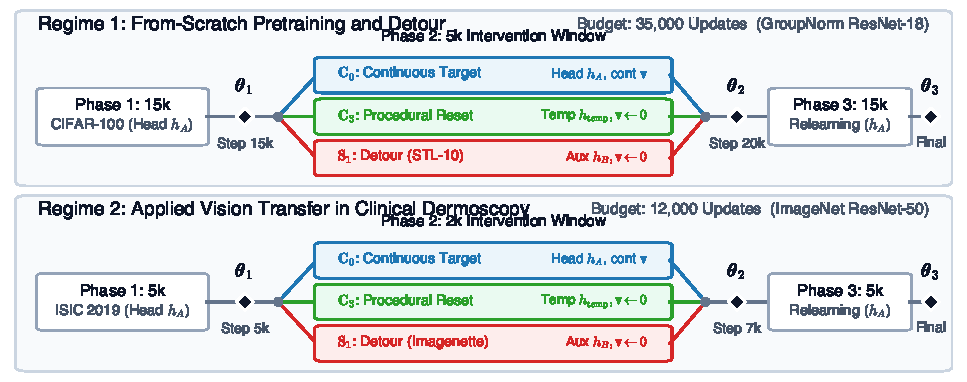
\includegraphics[width=0.72\linewidth]{figures/figure_edafnet_style_framework.pdf}
\caption{\textbf{Controlled Multi-Phase Experimental Protocols.} Three-phase schedules in the from-scratch and applied regimes. \newline (Top) Regime 1: from-scratch CIFAR-100 optimization with 35k updates. (Bottom) Regime 2: clinical dermoscopy fine-tuning on ISIC 2019 with 12k updates. Both compare continuous training ($C_0$, blue), on-target reset ($C_3$, green), and the auxiliary detour ($S_1$, red).}\label{fig:framework}
\end{figure*}


\subsection{State Management and Boundary Transition Rules}
\label{subsec:schedule_transitions}

For the $C_3$--$S_1$ comparison, transition procedures are held constant and the Phase 2 dataset is the main difference. We retain the learned backbone parameters $\bm{\theta}_{\mathrm{bb}}$ across phase boundaries without reinitialization and continue to update them according to $\bm{\theta}_{\mathrm{bb}}^{(t)} = \bm{\theta}_{\mathrm{bb}}^{(t-1)} - \eta \, \bm{v}_{\mathrm{bb}}^{(t)}$.

Both intervention arms store the target head $h_A$ at update $u_1$. During Phase 2, the stored head receives no updates: $C_3$ trains $h_{\mathrm{temp}}$ on target data, whereas $S_1$ trains $h_B$ on intermediate data. At $u_1 + u_B$, we discard these temporary heads and restore $h_A$. The target head in $C_0$ remains in place throughout.

Momentum vectors $\bm{v}$ in $C_0$ continue across both boundaries. We instead zero backbone momentum ($\bm{v}_{\mathrm{bb}} \leftarrow \mathbf{0}$) in $C_3$ and $S_1$ at $u_1$ and $u_1 + u_B$. When the target head returns for Phase 3, its saved momentum returns with it. The intervention arms thus share the head and momentum procedures despite their different Phase 2 datasets.

Regime 1 uses Group Normalization with $G = 32$ \cite{wu2018groupnorm}. Statistics are computed within each sample across channel groups, with no running batch averages. Switching datasets therefore cannot interfere through stored normalization statistics. Table~\ref{tab:intervention_matrix} summarizes the intervention configurations.


\begin{table*}[t]
\caption{Controlled multi-phase intervention matrix for the primary and ablation conditions. Within each seed block, all arms branch from the identical checkpoint $\bm{\theta}_1$.}\label{tab:intervention_matrix}
\centering
\resizebox{\linewidth}{!}{%
\begin{tabular}{l l l c ccc}
\toprule
\textbf{Schedule Arm} & \textbf{Phase 2 Dataset} & \textbf{Phase 2 Head} & \textbf{Momentum Reset} & \textbf{Target Updates} & \textbf{Aux Updates} & \textbf{Total Updates} \\
\midrule
$C_0$ (Continuous Baseline) & CIFAR-100 & Target $h_A$ (100 cls) & None (Continuous) & 35k & 0 & 35k \\
$C_0$ (30k Exposure Ctrl)  & CIFAR-100 & Target $h_A$ (100 cls) & None (Continuous) & 30k & 0 & 30k \\
$C_3$ (Procedural Reset)   & CIFAR-100 & Temp $h_{\mathrm{temp}}$ (100 cls) & At 15k, 20k ($\bm{v} \leftarrow \mathbf{0}$) & 35k & 0 & 35k \\
$S_1$ (Auxiliary Detour)    & STL-10    & Aux $h_B$ (10 cls) & At 15k, 20k ($\bm{v} \leftarrow \mathbf{0}$) & 30k & 5k & 35k \\
\bottomrule
\end{tabular}%
}
\end{table*}

\subsection{Formal Specification of Comparative Estimands}\label{subsec:schedule_estimands}

Four paired estimands distinguish compute budgets, target exposure, procedural resets, and inductive transfer effects:
\begin{align}
    \Delta_{\mathrm{total}} &\triangleq \mathrm{Acc}(S_1; 35\,\mathrm{k}) - \mathrm{Acc}(C_0; 35\,\mathrm{k}), \label{eq:delta_total} \\
    \Delta_{\mathrm{target}} &\triangleq \mathrm{Acc}(S_1; 35\,\mathrm{k}) - \mathrm{Acc}(C_0; 30\,\mathrm{k}), \label{eq:delta_target} \\
    \Delta_{\mathrm{proc}} &\triangleq \mathrm{Acc}(C_3; 35\,\mathrm{k}) - \mathrm{Acc}(C_0; 35\,\mathrm{k}), \label{eq:delta_proc} \\
    \Delta_{\mathrm{aux}} &\triangleq \mathrm{Acc}(S_1; 35\,\mathrm{k}) - \mathrm{Acc}(C_3; 35\,\mathrm{k}). \label{eq:delta_aux}
\end{align}


The $5{,}000$ updates spent on STL-10 replace CIFAR-100 training. For $\Delta_{\mathrm{total}}$, we compare $S_1$ and $C_0$ after $35{,}000$ total updates each; for $\Delta_{\mathrm{target}}$, we compare $S_1$ with $C_0$ at $30{,}000$ updates to give equal target exposure.

For $\Delta_{\mathrm{proc}}$, we compare $C_3$ with uninterrupted $C_0$: both train on CIFAR-100, but $C_3$ substitutes heads and resets momentum. For $\Delta_{\mathrm{aux}}$, we compare $S_1$ with $C_3$ at $35{,}000$ total updates under identical transitions. During Phase 2, $S_1$ trains on STL-10 and $C_3$ on CIFAR-100. This contrast estimates the effect of substituting auxiliary updates for target updates while keeping the procedural resets fixed, a contribution that the budget contrasts alone cannot separate.

\subsection{Mechanistic \texorpdfstring{$2 \times 2$}{2x2} Factorial Decomposition Protocol}\label{subsec:schedule_factorial}

Loss of accuracy in $C_3$ entails head replacement and clearing momentum. Since the extent to which the two contribute and interact is not known, each one of them is separated through the conduct of a $2 \times 2$ factorial experiment (complete crossing) using CIFAR-100 dataset ($N = 6$ paired seeds, 35,000 iterations) on the two factors. Head replacement will employ the binary factor $h \in \{0, 1\}$ where $h = 0$ preserves head $h_A$ while $h = 1$ replaces it.

Similarly, we parameterize momentum reset with a binary factor $m \in \{0, 1\}$, where $m = 0$ lets velocity vectors $\bm{v}_{\mathrm{bb}}$ flow continuously, and $m = 1$ zeroes velocity buffers ($\bm{v}_{\mathrm{bb}} \leftarrow \mathbf{0}$) at each boundary.

The combination of these two variables leads to four experimental conditions: continuous baseline $F_{00}$ ($C_0$), momentum resetting alone $F_{01}$, head replacement alone $F_{10}$, and controlled combination $F_{11}$ ($C_3$). Based on the mean accuracy $\mu_{hm}$ of all four experimental conditions, we determine the main effects of head replacement and momentum resetting, as well as their two-factor interaction:
\begin{align}
    \Delta_{\mathrm{head}} &\triangleq \frac{1}{2} \left[ (\mu_{10} - \mu_{00}) + (\mu_{11} - \mu_{01}) \right], \label{eq:factorial_head} \\
    \Delta_{\mathrm{mom}}  &\triangleq \frac{1}{2} \left[ (\mu_{01} - \mu_{00}) + (\mu_{11} - \mu_{10}) \right], \label{eq:factorial_mom} \\
    \Delta_{\mathrm{interaction}} &\triangleq (\mu_{11} - \mu_{01}) - (\mu_{10} - \mu_{00}). \label{eq:factorial_interaction}
\end{align}

\section{Experimental Setup and Analysis Protocol}\label{sec:protocol}


\subsection{Datasets, Preprocessing, and Split Partitions}
\label{subsec:protocol_datasets}

The Regime 1 target is CIFAR-100: $60{,}000$ color images of size $32 \times 32$ across 100 classes \cite{krizhevsky2009cifar}. We use $45{,}000$ images for backbone training and linear-probe fitting, $5{,}000$ for probe validation, and the remaining $10{,}000$ exclusively for final testing.

The auxiliary dataset is the labeled portion of STL-10, with $5{,}000$ images across 10 classes \cite{coates2011stl10}. We resize STL-10's higher-resolution images to the CIFAR-100 input size of $32 \times 32$ by bicubic interpolation. Both datasets receive random horizontal flips and random crops with four pixels of padding, keeping input dimensions and augmentation consistent across the target and auxiliary tasks.


\subsection{Network Architecture and Optimization Hyperparameters}
\label{subsec:protocol_model}

For Regime 1, we modify ResNet-18 \cite{he2016deep} to have input dimensions of $32 \times 32$, and we substitute batch normalization layers with Group Normalization layers ($G = 32$) \cite{wu2018groupnorm}. How this modification avoids statistics from getting stored while switching between CIFAR-100 and STL-10 datasets is elaborated in Section~\ref{subsec:schedule_transitions}. The final convolutional feature maps undergo adaptive averaging pooling that results in a 512-dimensional feature representation $\bm{z} \in \mathbb{R}^{512}$ followed by the linear classification layer $\bm{W}\bm{z} + \bm{b}$. For Regime 1, we use mini-batch stochastic gradient descent with a batch size of $B = 128$, momentum of $\mu = 0.9$, and weight decay of $5 \times 10^{-4}$. We keep the learning rate constant at $\eta = 0.1$ for $35{,}000$ steps without any learning rate decay or restarts.


\subsection{Diagnostic Representation Metrics}
\label{subsec:protocol_diagnostics}

Representation trajectory checkpoints are taken at step 15,000 ($\bm{\theta}_1$) before the auxiliary task phase; step 20,000 ($\bm{\theta}_2$) after the auxiliary task phase; and step 35,000 ($\bm{\theta}_3$) after the re-learning phase. Our three representation diagnostics include the linear probe which is used to measure CIFAR-100 class discrimination using a frozen backbone network. At each checkpoint, the backbone network is frozen and a different linear classifier is trained for its features \cite{alain2017understanding,belinkov2022probing}. The probe weights are $\bm{W}_{\mathrm{probe}} \in \mathbb{R}^{100 \times 512}$, where there are 100 classes in CIFAR-100 dataset and 512-dimensional embeddings. Each probe is trained for 5 epochs with Adam optimizer, learning rate of $\eta = 10^{-3}$ and weight decay of $10^{-4}$ and then evaluated on the validation split. The accuracy score of this probe gives an indication of the accessibility of target labels by the representation of backbone network.

Next, we measure the dimensionality of the learned representations using Effective Rank ($\EffRank$) \cite{roy2007effective,begga2026preserving}. For centered feature matrices $\bm{Z} \in \mathbb{R}^{N \times 512}$ extracted from $N = 2{,}000$ images, Effective Rank computes the exponential of the Shannon entropy of normalized singular values $p_k = \sigma_k / \sum_j \sigma_j$:
\begin{equation}\label{eq:effrank}
    \EffRank(\bm{Z}) \triangleq \exp\left( -\sum_{k=1}^r p_k \ln p_k \right) \in [1, 512].
\end{equation}
Values near 512 indicate that features spread evenly across the embedding space, whereas sharp drops signal dimensional collapse.

Finally, representation drift is measured by linear CKA with respect to baseline checkpoint $\bm{\theta}_1$ \cite{kornblith2019similarity}. Representation drift is quantified by $\Dcka \triangleq 1 - \mathrm{CKA}(\bm{Z}_{\mathrm{pre}}, \bm{Z}_t) \in [0, 1]$. Effective rank and CKA drift in tandem give us an insight into the nature of the representation drift as either a rigid coordinate rotation or loss of dimensions completely.

\subsection{Prespecified Paired Statistical Analysis Protocol}
\label{subsec:protocol_statistics}

$N=20$ seed pairs ranging from $920001$ to $920020$ are used for the confirmatory analysis in the Regime 1. The key comparison of interest is the contrast of the continuous training $C_0$ with respect to the auxiliary detour $S_1$, $d_s=\mathrm{Acc}(S_1;s)-\mathrm{Acc}(C_0;s)$. We test the hypothesis H1 using the two-sided paired Student's t-test with 19 degrees of freedom according to the pre-defined procedure described prior to the confirmatory runs. In addition to the paired t-test, we perform two additional checks under the different assumptions. Namely, we build the percentile bootstrap interval based on $10{,}000$ bootstrap samples and perform an exact sign flip permutation test by enumerating all possible $2^{20}=1{,}048{,}576$ sign permutations. The exploratory sample ($N=6$) and the confirmatory sample ($N=14$) are tested separately.


\section{Regime 1: From-Scratch Pretraining Results}\label{sec:results}

\subsection{Primary Confirmatory Evaluation: Resolving Hypothesis H1}\label{subsec:results_primary}

\begin{table*}[t]
\caption{Primary confirmatory inferential statistics on CIFAR-100 across $N = 20$ independent paired seeds on GroupNorm ResNet-18 under matched computational budget ($35{,}000$ updates).}\label{tab:primary_confirmatory}
\centering
\resizebox{\linewidth}{!}{%
\begin{tabular}{l ccccc c}
\toprule
\textbf{Contrast Estimand} & \textbf{Mean Diff.} & \textbf{Paired SD} & \textbf{95\% Paired $t$-CI} & $t(19)$ & $p$-value & Cohen's $d_z$ \\
\midrule
$\Delta_{\mathrm{total}} = S_1 - C_0$ (Primary H1) & $-0.43$ pp & 1.08 pp & [$-0.94$, $+0.07$] pp & $-1.79$ & 0.090 & $-0.40$ \\
$\Delta_{\mathrm{target}} = S_1 - C_0(30\mathrm{k})$ & $+0.27$ pp & 1.57 pp & [$-0.47$, $+1.00$] pp & $+0.76$ & 0.458 & $+0.17$ \\
$\Delta_{\mathrm{proc}} = C_3 - C_0$ (Procedural Reset) & $-0.40$ pp & 1.58 pp & [$-1.14$, $+0.34$] pp & $-1.14$ & 0.269 & $-0.25$ \\
$\Delta_{\mathrm{aux}} = S_1 - C_3$ (Data Contribution) & $-0.03$ pp & 1.56 pp & [$-0.76$, $+0.70$] pp & $-0.09$ & 0.933 & $-0.02$ \\
\bottomrule
\end{tabular}%
}
\end{table*}

\begin{figure*}[t]
\centering
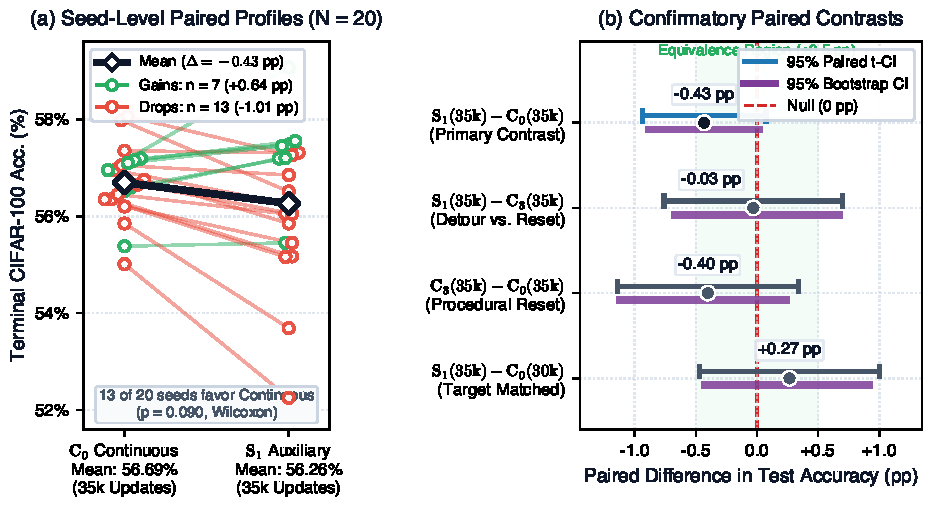
\includegraphics[width=0.76\linewidth]{figures/figure_paired_contrasts_forest_plot.pdf}
\caption{\textbf{Primary Paired Confirmatory Contrasts on CIFAR-100.} Auxiliary detours yield no significant transfer advantage over continuous training under matched budgets. \newline Mean paired differences across $N = 20$ seeds are shown with 95\% paired $t$-intervals (thick bars), 95\% bootstrap intervals (thin ticks), and individual differences (open circles) for the exploratory ($N = 6$) and confirmatory ($N = 14$) partitions.}\label{fig:confirmatory_forest}
\end{figure*}

We consider detour schedule $S_1$ relative to baseline $C_0$ using a matched budget of 35,000 updates to assess Hypothesis H1 over $N = 20$ paired random seeds. Continuous training results in a mean test accuracy of $56.69\% \pm 0.75\%$ for CIFAR-100, and $56.26\% \pm 1.51\%$ when a budget of 5,000 updates goes to STL-10. The main effect, $\Delta_{\mathrm{total}} = S_1 - C_0$, is $-0.43$ pp ($95\%$ paired $t$-interval [$-0.94$, $+0.07$] pp, $t(19) = -1.79$, $p = 0.090$; permutation $p = 0.091$; see Table~\ref{tab:primary_confirmatory}). Continuous training outperforms detour training in 13 of 20 seeds, and paired differences vary between $-2.76$ and $+2.12$ pp. Thus, the confidence interval precludes practical improvement, and the mean difference continues to be negative. These findings do not confirm Hypothesis H1 because it does not matter whether we invest resources on a detour or not.

The CIFAR-100 procedural control procedure $C_3$ incorporates the head swap and momentum reset of $S_1$ but without the use of any additional target data. Compared to uninterrupted training, the average difference is $-0.40$ pp ($95\%$ CI [$-1.14$, $+0.34$] pp, $t(19) = -1.14, p = 0.269$). The difference between the detour-minus-reset comparison, that is $\Delta_{\mathrm{aux}} = S_1 - C_3$, is $-0.03$ pp ($95\%$ CI [$-0.76$, $+0.70$] pp, $t(19) = -0.09, p = 0.933$). Given that the procedural resets are constant, the auxiliary STL-10 images have contributed no transfer value whatsoever, either positive or negative. This is confirmed by Figure~\ref{fig:confirmatory_forest} where we see essentially zero transfer value both in the early exploratory sample of size six, where the difference was $-0.89$ pp, and in the confirmatory sample of size 14, where the difference was $-0.24$ pp.

\subsection{Factorial Decomposition of the Procedural Reset Penalty}\label{subsec:results_procedural}

\begin{table*}[t]
\caption{Mechanistic $2 \times 2$ factorial decomposition of procedural reset components on CIFAR-100 ($N = 6$ paired seeds, $35{,}000$ updates). All arms fork from checkpoint $\bm{\theta}_1$ at step $15{,}000$.}\label{tab:factorial_summary}
\centering
\resizebox{\linewidth}{!}{%
\begin{tabular}{l l l c}
\toprule
\textbf{Factorial Arm} & \textbf{Head Policy ($h$)} & \textbf{Momentum Policy ($m$)} & \textbf{Terminal Test Accuracy (\%)} \\
\midrule
$F_{00}$ ($C_0$ Baseline) & Retained target $h_A$ & Continuous carryover & $56.32 \pm 1.13$ \\
$F_{01}$ (Momentum Reset Only) & Retained target $h_A$ & Zeroed at boundaries ($\bm{v} \leftarrow \mathbf{0}$) & $56.88 \pm 0.86$ \\
$F_{10}$ (Head Substitution Only) & Temporary head $h_{\mathrm{temp}}$ & Continuous carryover & $54.21 \pm 1.21$ \\
$F_{11}$ ($C_3$ Bundled Reset) & Temporary head $h_{\mathrm{temp}}$ & Zeroed at boundaries ($\bm{v} \leftarrow \mathbf{0}$) & $54.79 \pm 1.32$ \\
\midrule
\multicolumn{4}{l}{\textbf{Repeated-Measures ANOVA and Marginal Contrast Estimates ($5$ degrees of freedom):}} \\
\multicolumn{2}{l}{Main effect of head substitution ($\Delta_{\mathrm{head}}$)} & \multicolumn{2}{c}{$-2.10$ pp ($95\%$ CI: [$-3.18$, $-1.02$] pp, $F = 24.95, p = 0.004$)} \\
\multicolumn{2}{l}{Main effect of momentum clearing ($\Delta_{\mathrm{mom}}$)}   & \multicolumn{2}{c}{$+0.57$ pp ($95\%$ CI: [$-0.64$, $+1.77$] pp, $F = 1.47, p = 0.279$)} \\
\multicolumn{2}{l}{Factorial interaction ($\Delta_{\mathrm{interaction}}$)}      & \multicolumn{2}{c}{$+0.02$ pp ($95\%$ CI: [$-1.25$, $+1.29$] pp, $F = 0.002, p = 0.967$)} \\
\bottomrule
\end{tabular}%
}
\end{table*}

\begin{figure*}[t]
\centering
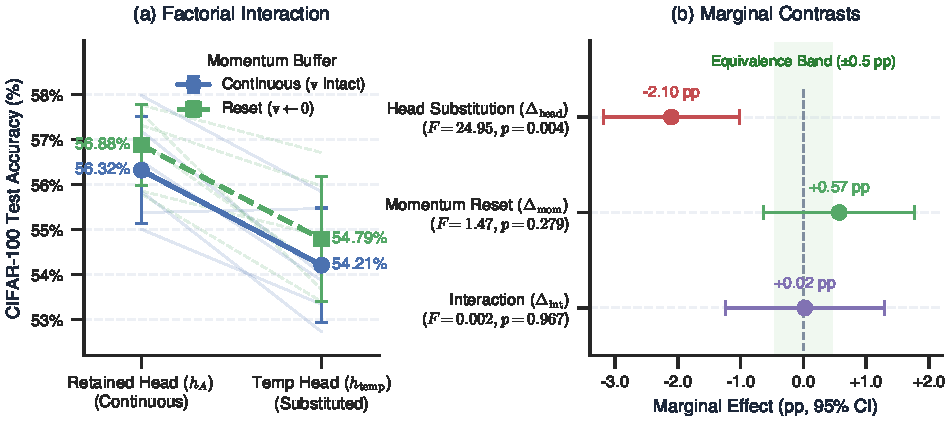
\includegraphics[width=0.74\linewidth]{figures/figure_factorial_decomposition.pdf}
\caption{\textbf{Factorial Attribution of Procedural Reset Penalties.} Head replacement accounts entirely for the observed transfer deficit, while momentum flushing provides mild regularization. \newline (a) Interaction plot showing strictly parallel trajectories across the four factorial arms, indicating zero interaction ($+0.02$ pp, $p = 0.967$). (b) Marginal main effects forest plot confirming a significant head penalty ($-2.10$ pp, $p = 0.004$) versus an uncertain momentum effect ($+0.57$ pp, $p = 0.279$).}\label{fig:factorial_decomposition}
\end{figure*}


The summary of the $2 \times 2$ factorial design with $N = 6$ paired seeds for breaking down the head and momentum factors into the procedural reset control ($C_3$) is provided in Table~\ref{tab:factorial_summary} and Figure~\ref{fig:factorial_decomposition}. Head replacement leads to a larger contribution of $\Delta_{\mathrm{head}} = -2.10$ percentage points in terms of average accuracy decrease ($F(1,5) = 24.95$, $p = 0.004$). Momentum clearing ($\bm{v} \leftarrow \mathbf{0}$) leads to an average effect equal to $\Delta_{\mathrm{mom}} = +0.57$ pp ($F(1,5) = 1.47$, $p = 0.279$). Such a positive estimate of the effect does not imply its consistency. The nearly parallel lines in Figure~\ref{fig:factorial_decomposition}a agree with a small interaction effect of $\Delta_{\mathrm{interaction}} = +0.02$ pp ($F(1,5) = 0.002$, $p = 0.967$). Based on these results, head substitution appears to be the more significant factor in the procedural penalty. However, the interaction estimate is not sufficient evidence for claiming independence of the operations.

\subsection{Longitudinal Representation Trajectory Dynamics}\label{subsec:results_representations}

\begin{table*}[t]
\caption{Longitudinal representation dynamics on CIFAR-100 across milestones $\bm{\theta}_1$ (step 15k), $\bm{\theta}_2$ (step 20k), and $\bm{\theta}_3$ (step 35k) ($N = 10$ seeds, GroupNorm ResNet-18).}\label{tab:representation_geometry}
\centering
\resizebox{\linewidth}{!}{%
\begin{tabular}{l ccc ccc cc}
\toprule
& \multicolumn{3}{c}{\textbf{Matched Frozen Probe (\%)}} & \multicolumn{3}{c}{\textbf{Effective Rank ($\EffRank \in [1, 512]$)}} & \multicolumn{2}{c}{\textbf{CKA Drift ($\Dcka$)}} \\
\cmidrule(lr){2-4} \cmidrule(lr){5-7} \cmidrule(lr){8-9}
\textbf{Condition} & $\bm{\theta}_1$ & $\bm{\theta}_2$ & $\bm{\theta}_3$ & $\bm{\theta}_1$ & $\bm{\theta}_2$ & $\bm{\theta}_3$ & $\bm{\theta}_2$ & $\bm{\theta}_3$ \\
\midrule
$C_0$ (Continuous) & $52.8 \pm 0.9$ & --- & $63.0 \pm 0.9$ & $162.7 \pm 7.4$ & --- & $160.7 \pm 9.4$ & --- & $0.320 \pm 0.025$ \\
$C_3$ (Reset Ctrl) & $52.8 \pm 0.9$ & $60.9 \pm 0.9$ & $63.0 \pm 1.0$ & $162.7 \pm 7.4$ & $165.4 \pm 8.9$ & $160.8 \pm 7.9$ & $0.220 \pm 0.012$ & $0.334 \pm 0.028$ \\
$S_1$ (Auxiliary)  & $52.8 \pm 0.9$ & $21.9 \pm 1.1$ & $62.7 \pm 0.9$ & $162.7 \pm 7.4$ & $122.9 \pm 5.9$ & $152.0 \pm 8.2$ & $0.655 \pm 0.034$ & $0.461 \pm 0.038$ \\
\bottomrule
\end{tabular}%
}
\end{table*}

\begin{figure*}[t]
\centering
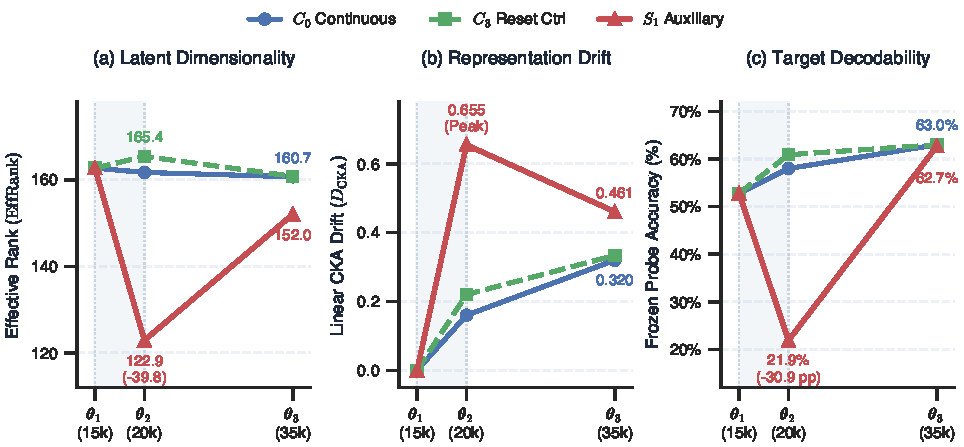
\includegraphics[width=0.76\linewidth]{figures/figure_longitudinal_representation_dynamics.pdf}
\caption{\textbf{Longitudinal Representation Trajectory Dynamics on CIFAR-100.} Off-task gradients induce severe representational distortion that is rapidly repaired during target relearning. \newline (a) Effective Rank contracting during auxiliary training at $\bm{\theta}_2$ before recovering during Phase 3. (b) Linear CKA drift showing persistent representational rotation at $\bm{\theta}_3$ ($\Dcka = 0.461$). (c) Matched frozen linear probes collapsing to $21.9\%$ under the detour before snapping back to statistical parity with $C_0$ ($62.7\%$).}\label{fig:representation_dynamics}
\end{figure*}

We follow linear probe accuracy, Effective Rank ($\EffRank$), and linear CKA drift ($\Dcka$) through $\bm{\theta}_1$ (step 15k), $\bm{\theta}_2$ (step 20k), and $\bm{\theta}_3$ (step 35k) in Table~\ref{tab:representation_geometry} and Figure~\ref{fig:representation_dynamics}.

By the end of Phase 2 ($\bm{\theta}_2$), STL-10 training has heavily reshaped the feature space. CIFAR-100 probe accuracy collapses from $52.8\%$ to $21.9\%$ ($s = 1.1\%$). Effective Rank falls from $162.7$ to $122.9$ ($s = 5.9$). CKA drift from $\bm{\theta}_1$ rises to $\Dcka = 0.655$ ($s = 0.034$). The on-target reset control ($C_3$) shows no such disruption: probe accuracy remains high ($60.9\% \pm 0.9\%$), dimensionality remains full ($165.4 \pm 8.9$), and representation drift is small ($\Dcka = 0.220 \pm 0.012$).

Separability recovers quickly upon returning to CIFAR-100 in Phase 3 training. Probe accuracy for $S_1$ at update 35,000 ($\bm{\theta}_3$) is $62.7\% \pm 0.9\%$, very similar to $C_0$ ($63.0\% \pm 0.9\%$) and reset control $C_3$ ($63.0\% \pm 1.0\%$). Effective rank recovers to $152.0 \pm 8.2$. The separation of classes recovers but the geometry of the network has been irreversibly distorted such that the drift in final CKA remains high at $\Dcka = 0.461 \pm 0.038$, significantly greater than $0.320 \pm 0.025$ for $C_0$. The retraining on the target task does not nudge weights back onto their original trajectory but learns new boundaries in a distorted coordinate system.

\subsection{Multi-Domain Screening Spectrum and Architectural Generality}\label{subsec:results_screening_spectrum}

Phase 2 screening includes 6 different conditions with $N=5$ seeds each (Figure~\ref{fig:screening_spectrum}). In addition to the continuous training and clean reset conditions $B_0$ and $B_1$, we perform four additional conditions: CIFAR-10 $B_3$, STL-10 $B_4$, SVHN $B_5$, and Gaussian noise $B_7$. This STL-10 shift comparison is extended to other image conditions. Overall, among the natural image conditions, an increased Phase 2 CKA drift is correlated with a validation accuracy drop. The Gaussian noise is especially harmful in terms of Phase 2 CKA drift, where the Effective Rank goes down to $\EffRank \to 124.5$. To recover performance on the target task, the Gaussian noise requires $u_{\mathrm{rec}} = 4{,}820$ updates.




\begin{figure*}[t]
\centering
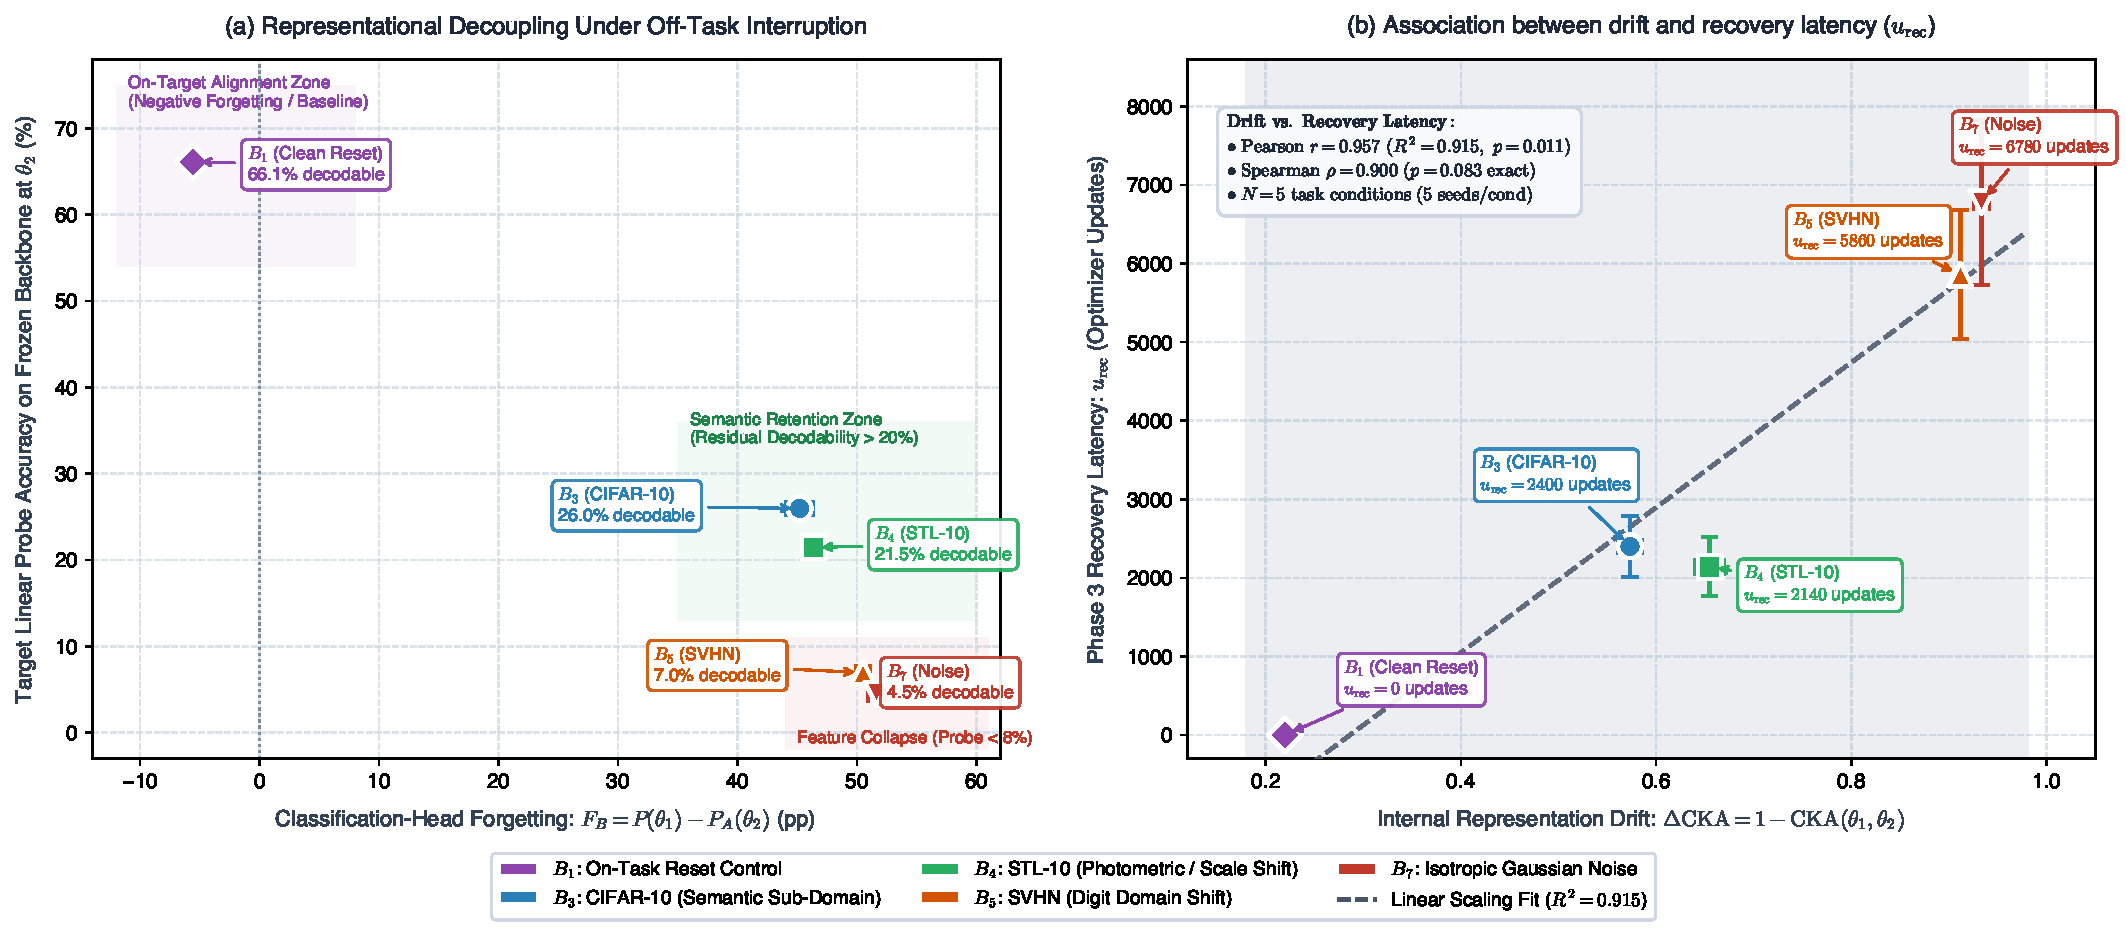
\includegraphics[width=0.76\linewidth]{figures/figure_monotonic_representation_spectrum.pdf}
\caption{\textbf{Multi-Domain Representation and Recovery Spectrum.} Target relearning latency scales monotonically with geometric representational displacement. \newline (a) Monotonic relationship between recovery latency ($u_{\mathrm{rec}}$) and Phase 2 linear CKA drift across natural and synthetic shifts ($B_1$ to $B_7$). (b) Validation performance drop tracking geometric representational drift across the full semantic spectrum.}\label{fig:screening_spectrum}
\end{figure*}


\paragraph{Ablations and Architectural Generality (CViT):}

We introduce variations to detouring by changing its start from steps 10k to 15k and the length of the detour from 2.5k to 5k updates. A long detour disturbs the representation more, but the models recover due to subsequent training with the target. We compare our architectures in the next table.

The architecture comparison uses an 8-layer Compact Vision Transformer (CViT) with five random seeds. Continuous training reaches 43.77\% accuracy and the auxiliary detour 43.71\%, a $-0.06$ percentage point difference ($p = 0.806$). The small terminal difference suggests that the absence of a clear detour advantage extends beyond the ResNet architecture tested earlier. The five-seed comparison alone does not establish identical representation dynamics across architectures. Model configurations and individual seed results appear in Supplementary Material Sections C-E.


\section{Regime 2: Applied Vision Fine-Tuning in Clinical Dermoscopy}\label{sec:applied_finetuning}

We examine these optimization dynamics in clinical skin lesion diagnosis by fine-tuning an ImageNet-pretrained ResNet-50 at $224 \times 224$ resolution on ISIC 2019. The dataset contains 25,331 dermoscopy images across 8 diagnostic categories \cite{codella2018skin,tschandl2018ham10000}. The auxiliary task uses Imagenette, a 10-class natural image subset of ImageNet \cite{howard2020fastai}.

\subsection{Applied Protocol Specification}\label{subsec:applied_protocol}
We divide exactly 12,000 parameter updates into three stages. Phase 1 trains on ISIC 2019 for $u_1 = 5{,}000$ updates with primary head $\mathrm{Head}_A$. In Phase 2, four parallel conditions receive $u_B = 2{,}000$ updates: continuous target fine-tuning ($C_0$), on-target procedural reset ($C_3$), an Imagenette detour ($S_1$), and a label-shuffled Imagenette detour ($S_1\text{-shuf}$). All models then complete $u_2 = 5{,}000$ further ISIC 2019 updates in Phase 3.

All backbones start from the standard ImageNet-pretrained ResNet-50 weights (\texttt{IMAGENET1K\_V2}) \cite{he2016deep,wightman2021resnet}. At update 5,000, we freeze and store target head $\mathrm{Head}_A$ and its momentum buffers in memory, preventing corruption of these parameters during Phase 2. An initial two-seed pilot experiment confirmed that procedural reset effects replicate in this applied setting: control $C_3$ initially outperformed continuous training $C_0$ by $+0.82$ pp, whereas auxiliary detour $S_1$ showed a $-0.75$ pp deficit (Supplementary Section F).

\subsection{Primary Confirmatory Cohort on ISIC 2019}\label{subsec:applied_confirmatory}

\begin{table*}[t]
\caption{Primary confirmatory inferential statistics for applied vision fine-tuning on ISIC 2019 across $N = 8$ independent paired seeds ($12{,}000$ updates, ImageNet-pretrained ResNet-50).}\label{tab:applied_primary_confirmatory}
\centering
\resizebox{\linewidth}{!}{%
\begin{tabular}{l ccccc c}
\toprule
\textbf{Contrast Estimand} & \textbf{Mean Diff.} & \textbf{Paired SD} & \textbf{95\% Paired $t$-CI} & $t(7)$ & $p$-value & Cohen's $d_z$ \\
\midrule
$C_3 - C_0$ (Procedural Reset) & $-0.49$ pp & 1.01 pp & [$-1.34$, $+0.35$] pp & $-1.38$ & 0.209 & $-0.49$ \\
$S_1 - C_3$ (Detour vs. Reset Control) & $+0.08$ pp & 0.73 pp & [$-0.53$, $+0.69$] pp & $+0.31$ & 0.767 & $+0.11$ \\
$S_1 - C_0$ (Detour vs. Continuous Baseline) & $-0.41$ pp & 1.08 pp & [$-1.31$, $+0.49$] pp & $-1.08$ & 0.317 & $-0.38$ \\
\bottomrule
\end{tabular}%
}
\end{table*}

\begin{figure*}[t]
\centering
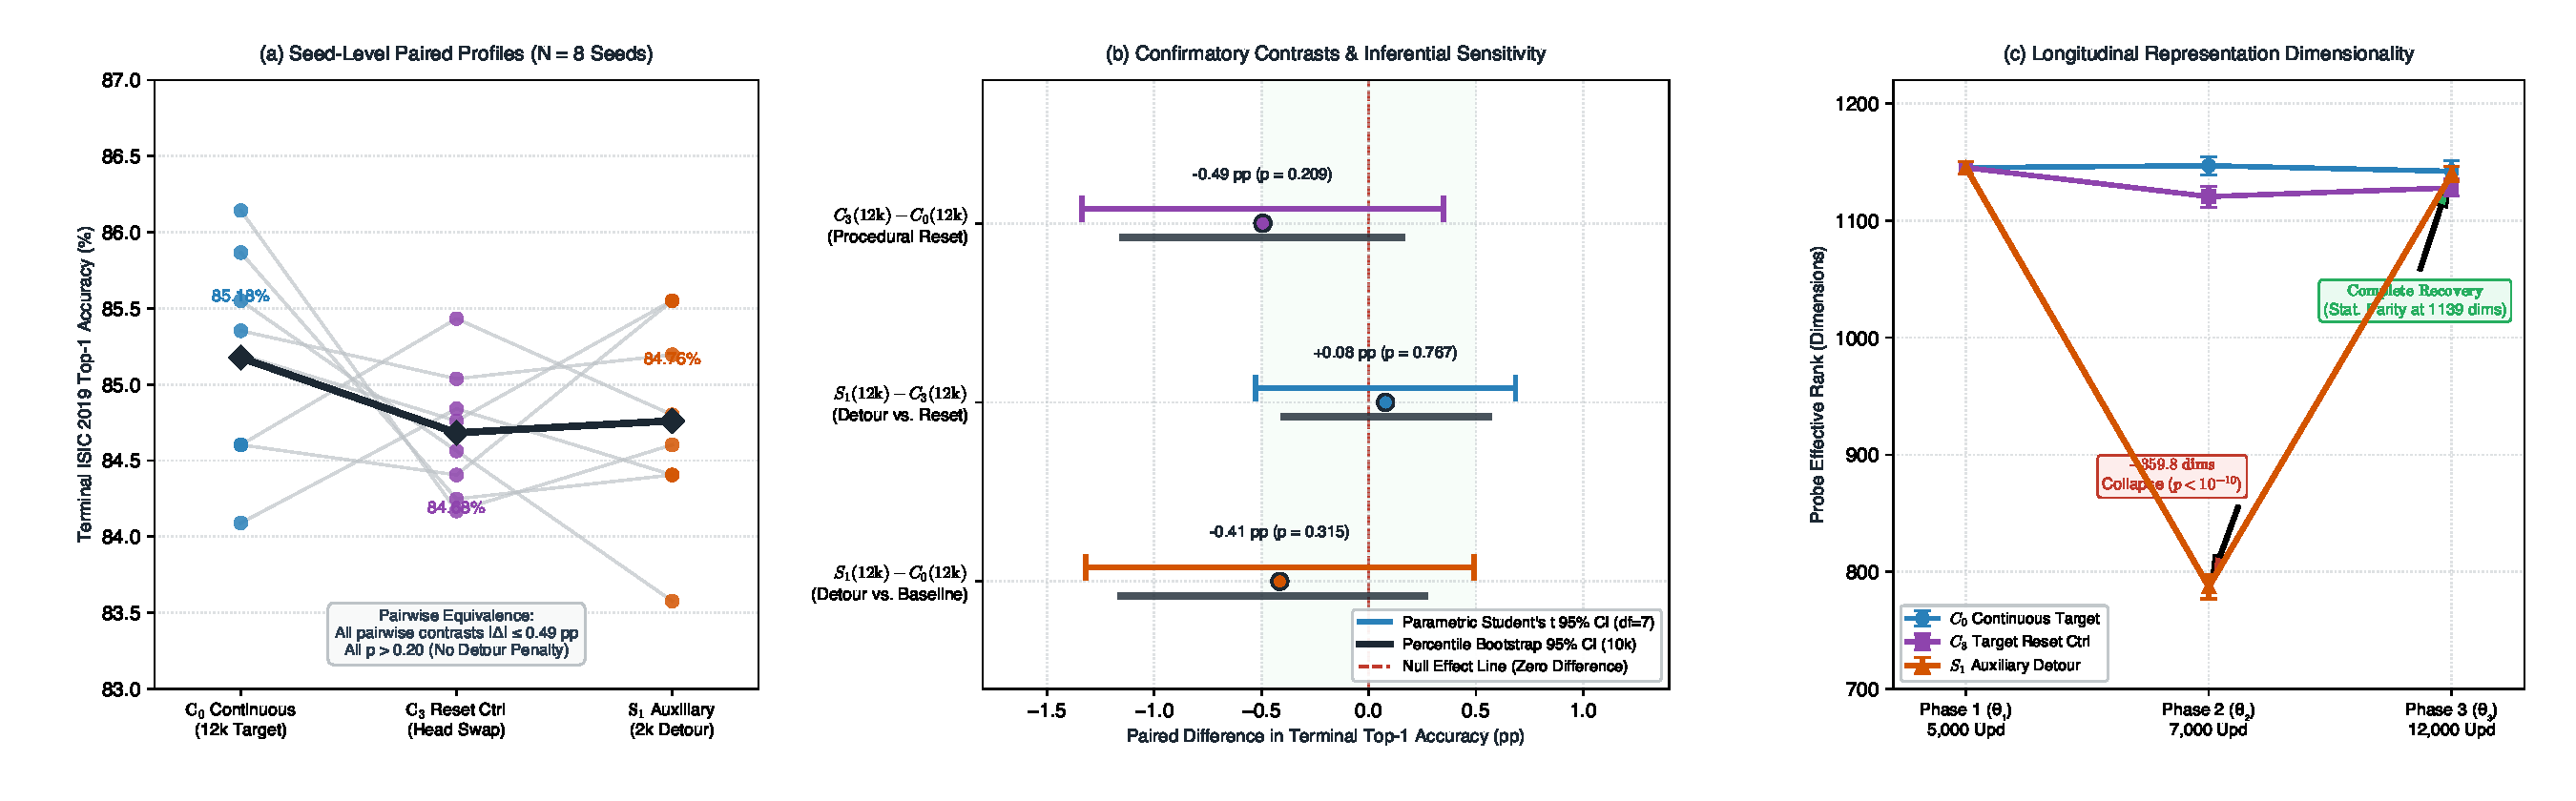
\includegraphics[width=0.70\linewidth]{figures/figure_applied_contrasts_forest_plot.pdf}
\caption{\textbf{Confirmatory Paired Contrasts in Applied Clinical Transfer.} Off-task natural image detours achieve statistical parity with procedural reset controls on clinical dermoscopy. \newline Mean paired differences across $N = 8$ seeds ($12{,}000$ updates, ImageNet ResNet-50) are shown with 95\% paired $t$-intervals (thick bars), 95\% bootstrap intervals (thin ticks), and individual paired differences (open circles). Both reset and detour arms yield null differences against baseline ($p > 0.20$).}\label{fig:applied_forest}
\end{figure*}

Across $N = 8$ paired random seeds (1001 to 1008), we compare continuous training ($C_0$), procedural reset ($C_3$), and the auxiliary detour ($S_1$). These 24 complete training runs test the benefit of detours on high-resolution medical data (Table~\ref{tab:applied_primary_confirmatory}, Figure~\ref{fig:applied_forest}).

On ISIC 2019, continuous fine-tuning reaches $85.18\% \pm 0.70\%$ Top-1 test accuracy, the procedural reset ($C_3$) reaches $84.68\% \pm 0.42\%$, and the 2,000-update Imagenette detour ($S_1$) reaches $84.76\% \pm 0.67\%$.

The detour-minus-continuous contrast ($\Delta_{\mathrm{total}} = S_1 - C_0$) is $-0.41$ percentage points ($95\%$ CI [$-1.31$, $+0.49$] pp, $t(7) = -1.08, p = 0.317$). Against the reset control ($S_1 - C_3$), the difference is $+0.08$ pp ($95\%$ CI [$-0.53$, $+0.69$] pp, $t(7) = +0.31, p = 0.767$). In realistic fine-tuning pipelines, taking an off-task detour neither improves nor harms final diagnostic accuracy; it performs essentially the same as an on-target procedural reset.

\subsection{Representation Dynamics: Transient Collapse vs. Asymptotic Plasticity}\label{subsec:applied_geometry}

\begin{figure*}[t]
\centering
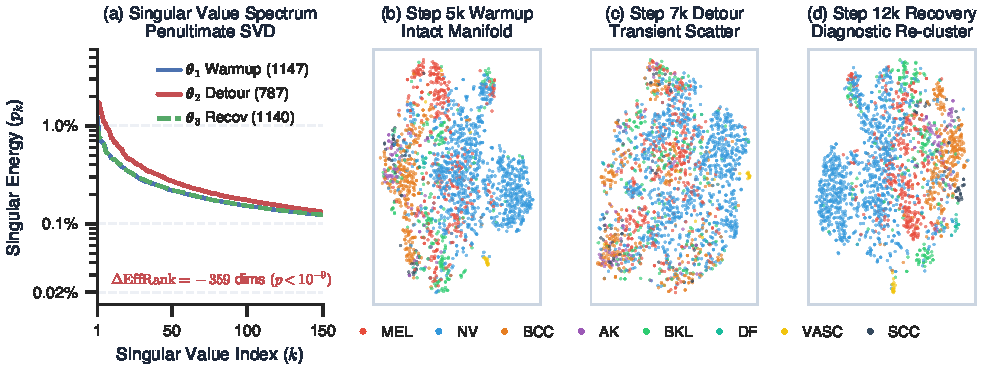
\includegraphics[width=0.68\linewidth]{figures/figure_applied_manifold_and_scree.pdf}
\caption{\textbf{Transient Representation Collapse and Asymptotic Recovery in Clinical Dermoscopy.} Representation geometry undergoes catastrophic compression during off-task detours but is fully restored under target relearning. \newline (a) Singular value spectrum showing transient spectral compression at $\bm{\theta}_2$ (red) and complete recovery at $\bm{\theta}_3$ (green). (b) Cumulative spectral energy demonstrating variance collapse. (c--f) 2D t-SNE projections of clinical test lesions across 8 ISIC categories. (c) Intact manifolds at $\bm{\theta}_1$; (d) Severe manifold rotation under the $S_1$ detour at $\bm{\theta}_2$; (e) Preserved manifolds under continuous $C_0$; (f) Diagnostic re-clustering at terminal $\bm{\theta}_3$.}\label{fig:applied_manifold_scree}
\end{figure*}

Penultimate layer activations are evaluated for 2,000 clinical test images at steps 5k ($\bm{\theta}_1$, after the warm-up), 7k ($\bm{\theta}_2$, end of the detour) and 12k ($\bm{\theta}_3$, final model). Geometry is characterized using singular value decomposition, Effective Rank, and two-dimensional t-SNE representations at each of these milestones (Figure~\ref{fig:applied_manifold_scree}). Effective rank decreases by 359 dimensions from $1146.9 \pm 8.3$ at step 5k to $787.1 \pm 10.9$ at step 7k ($t(7) = -53.4, p = 2.1 \times 10^{-11}$) during the second phase. CKA drift with respect to the warm-up checkpoint triples to $\Dcka = 0.476 \pm 0.032$, whereas continuous training with $C_0$ results in only $0.153 \pm 0.010$. Gradient updates in natural images cause quick distortion of feature representation in the medical domain. Figure~\ref{fig:applied_manifold_scree}d shows how off-task gradient updates affect feature space: representations get rotated away from the medical domain, with formerly separated classes of diagnostic lesions scattered.

By step 12,000 ($\bm{\theta}_3$), Effective Rank under $S_1$ has expanded to $1152.0 \pm 7.1$ dimensions, fully matching continuous training $C_0$ ($1153.4 \pm 9.7$). Resuming target training during Phase 3 repairs this internal disruption completely. Two-dimensional t-SNE plots (Figure~\ref{fig:applied_manifold_scree}f) confirm that lesion representations re-organize into distinct diagnostic clusters. Returning to target fine-tuning restores both internal representation geometry and final diagnostic accuracy after intermediate detours temporarily disrupt feature alignment, showing that pretrained networks have wide optimization basins.


\section{Implications and Limitations}
\label{sec:discussion}

\paragraph{Feature Recovery and Target Generalization:}
Accuracy on the final test was $56.26\%$ for the auxiliary schedule versus $56.69\%$ for the continuous baseline, despite the recovery of the target features. During the STL-10 detour, the probe accuracy for CIFAR-100 was down to $21.9\%$ and Effective Rank to 122.9, revealing significant alteration of the target features. Once the CIFAR-100 training was continued, probe accuracy went up to $62.7\%$, versus $63.0\%$ in the case of the continuous training, and the Effective Rank rose to 152.0. Thus, class separability was recovered significantly, although not implying full recovery of the original representation. Final test accuracy did not improve accordingly, showing that recovering linearly accessible target information is not equivalent to better generalization. The Compact Vision Transformer results (Supplementary Material Table~S7) provide additional support from the architecture perspective; future work should determine the generality of such representation dynamics.

\paragraph{Explaining Procedural Costs:}
In the framework of the six-seed factorial experiment, the head substitution corresponds to the effect of $-2.10$ percent ($p=0.004$), meaning that it is an important factor influencing procedural costs in this case. Head target that is saved returns to the modified backbone owing to the intermediary process of training and, hence, affects the backbone-classifier connection. Further optimization may be required to improve the relation between the two. Momentum clear has a positive effect but with not much statistical importance ($+0.57$ pp, $p=0.279$). The estimation of interaction is statistically insignificant ($+0.02$ pp, $p=0.967$); hence, there is no independence in this case. In other words, it is required to carry out procedural control to evaluate the impact of auxiliary data.

\paragraph{Practical Limits and Next Steps:}
However, the 5,000-image STL-10 database provided no increase in terminal accuracy within the fixed update budget framework. There is still a chance that there would be an increase in efficiency with larger databases, more complex task relations, or other divisions of the training period, since our results are constrained by the auxiliary databases, architectures, and schedules used. Clinical fine-tuning revealed that target training after significant intermediate interruption restored a large number of features measured, with final accuracy close to procedural controls. However, the sustainability of feature recovery along with final accuracy close to procedural controls is debatable beyond longer detours and other medical image databases.



Parameter-efficient adaptation could limit boundary disruption and thereby reduce the need for later recovery. With low-rank adaptation (LoRA), for example, the target classification interface could be retained while other components are adapted. Lower transition costs under this proposed adaptation would still need to be established with compute-matched and procedural controls.



\section{Conclusion}
\label{sec:conclusion}

For the both the from scratch and clinical test schedules, the detours did not enhance the accuracy of the targets in a matched update budget environment. The on target controls account for the effect of the auxiliary information alone and indicate that the boundary information is important too. The experimental design yielded an accuracy effect for head replacement greater than that of the momentum clearing effect, which was still ambiguous. Target training helped in regaining access to information that had been lost through off task changes in features. Yet, similar terminal accuracies do not necessarily mean the same representations.


\paragraph{Broader Impact Statement:}
Final accuracies hide significant shifts that can happen at intermediary checkpoints. An example from our clinical study is provided by the fact that the representation of ISIC 2019 undergoes a big change while doing the Imagenette detour task and recovers while target training. These results do not represent the clinical performance of the model at the intermediate checkpoint. Clinical models have to be validated for clinical performance at proper checkpoints. The benchmark datasets used in our experiments are CIFAR-100, STL-10, ISIC 2019, and Imagenette.

\paragraph{Reproducibility Statement:}
The schedules, update budgets, and optimization settings are documented in Sections~\ref{sec:schedules}, \ref{sec:protocol}, and \ref{sec:applied_finetuning}. The Supplementary Material provides individual seed logs, bootstrap distributions, and ANOVA tables for independent examination and replication.
 Anonymized code, training scripts, and run logs are publicly available at \url{https://anonymous.4open.science/r/off-task-learning-intervals-0B5C/}.

{\footnotesize
\setlength{\bibsep}{0pt}
\bibliography{references}
\bibliographystyle{tmlr}
}

\end{document}
